\section{Results}\label{sec:results}

We trained our method to optimize the insertion process in simulation as well as on physical hardware.
This section provides the results of our discussed experiments and shows the functionality of our method.

\subsection{Sample Efficiency of Residual RL}

First, we compare residual RL and pure RL without a hand-engineered controller on the insertion task. 
Fig. \ref{fig:fig2} shows in simulation and real-world that residual RL achieves a better final performance and requires less samples than RL alone, both in simulation and on physical hardware. 
Unlike residual RL, the pure RL approach needs to learn the structure of the position control problem from scratch, which explains the difference in sample efficiency.
As samples are expensive to collect in the real world, residual RL is better suited for solving real-world tasks. Moreover, RL shows a broader spatial variance during training and needs to explore a wider set of states compared to residual RL, which can be potentially dangerous in hardware deployments.

\begin{figure*}[t]
    \vspace{6pt}
    \centering
    \begin{subfigure}[b]{0.32\linewidth}
        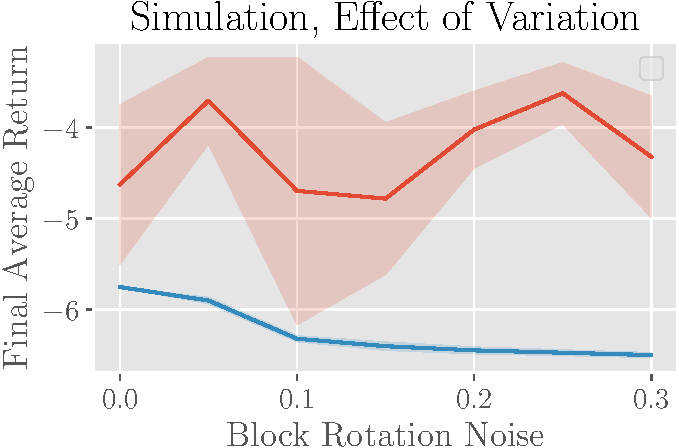
\includegraphics[width=0.99\linewidth]{residualrl/figs/env_variance_sim.pdf} \\
        \centering
        (a)
    \end{subfigure}
    \begin{subfigure}[b]{0.32\linewidth}
        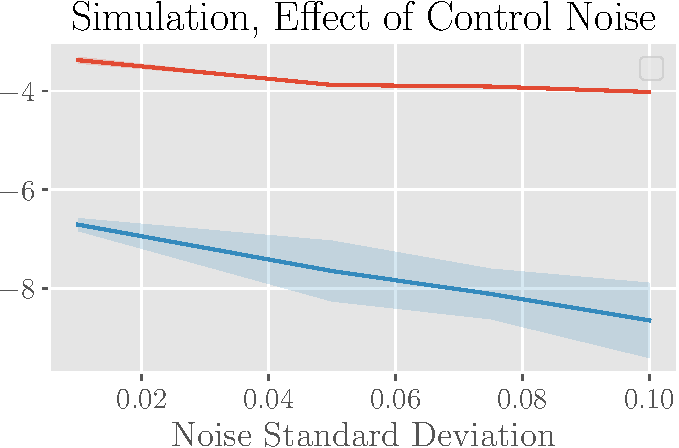
\includegraphics[width=0.99\linewidth]{residualrl/figs/control_noise_sim.pdf} \\
        \centering
        (b)
    \end{subfigure}
    \begin{subfigure}[b]{0.32\linewidth}
        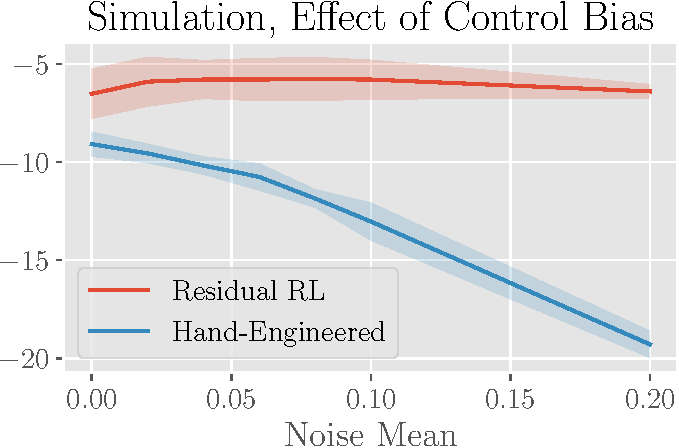
\includegraphics[width=0.99\linewidth]{residualrl/figs/control_bias_sim.pdf} \\
        \centering
        (c)
    \end{subfigure}
    \caption{Simulation results for different experiments. In each plot, the final average return obtained by running the method for various settings of a parameter is shown. Plot (a) shows that residual RL can adjust to noise in the environment caused by rotation of the blocks in a range of $0$ to $0.3$\,rad. In plot (b), residual RL finds robust strategies in order to reduce the effect of control noise, as the final average return is not greatly affected by the magnitude of noise. Plot (c) shows that residual RL can compensate for biased controllers and maintains good performance as control bias increases, while the performance of the hand-designed controller dramatically deteriorates with higher control bias.} %
    \label{fig:control_bias}
\end{figure*}

\subsection{Effect of Environment Variation}

In previous set of experiments, both standing blocks were placed in their initial position without any position or orientation error. 
In this case, the hand-engineered controller performs well, as both blocks are placed such that there is a sufficiently large defined gap for insertion. 
However, once the initial orientation of the blocks is randomized, the gap between the blocks and the goal position does not afford directly inserting from above.
Therefore, the hand-engineered controller struggles to solve the insertion task, succeeding in only 2/20 trials, while residual RL still succeeds in 15/20 trials. These results are summarized in Fig. \ref{fig:environment_variation}\,(a). Rollouts from the learned policy are included in \ref{fig:fig1}. In this experiment, the agent demonstrably learns consistent small corrective feedback behaviors in order to slightly nudge the blocks in the right direction without tipping them over, a behavior that is very difficult to manually specify.

The result of this experiment showcases the strength of residual RL. Since the human controller specifies the general trajectory of the optimal policy, environment samples are required only to learn this corrective feedback behavior. The real-world learning curve for the experiment in Fig. \ref{fig:environment_variation}\,(b) shows that this behavior is gradually acquired over the course of eight thousand samples, which is only about three hours of real-world training time.

We further studied the effect of the block orientation changing after every reset in simulation. The results are shown in Fig. \ref{fig:control_bias}\,(a). 
The simulation results show that the performance of the hand-engineered controller decreases as the block rotation angle increases, whereas our control method maintains a constant average performance over different variations. 

\subsection{Recovering from Control Noise}

In this experiment, we observe that residual RL is able to cope with actuator noise, including biased actuator noise.
Quantitative results for simulation are shown in  Fig.~\ref{fig:control_bias}\,(b) and (c). In Fig.~\ref{fig:control_bias}\,(c) our method keeps the average return constant and correct for biased controllers even as control bias increases, whereas the hand-engineered controller cannot compensate biased input and its performance deteriorates as control bias increases.
The same applies for adding control noise to the control output as shown in Fig.~\ref{fig:control_bias}\,(b).

For the hardware experiments, only biased actuator noise is investigated. These results are shown in Fig.~\ref{fig:environment_variation}\,(c). These learning curves show that even as more control bias is introduced, training in the real world proceeds without significant issues. This result suggests the potential for RL to address practical issues in automation such as sensor drift.

\subsection{Sim-to-Real with Residual RL}

The result of the sim-to-real experiment is shown in Fig. \ref{fig:sim_to_real}. In this experiment, each setting was run with three random seeds. Adding policy initialization from simulation significantly speeds up both RL and residual RL. In particular, residual RL with policy initialization from simulation successfully solves the task extremely quickly: in under one thousand timesteps of environment interaction. This method poses a highly sample efficient, practical way to solve robotics problems with  difficult contact dynamics.

\section{Related Work}\label{sec:related_work}

Reinforcement learning for robotics holds the promise of greater autonomy and reliability, which could be vital to improving our manufacturing processes beyond its current limitations.
RL methods have been difficult to apply in robotics because of sample efficiency, safety, and stability issues. Still, RL has been used to allow robots to learn tasks such as playing table tennis \cite{peters2010reps}, swinging up a cartpole and balancing a unicycle \cite{deisenroth2011pilco}, grasping~\cite{pinto2017robust, levine2017grasping}, opening a door \cite{Gu2016b}, and general manipulation tasks \cite{levine2016gps, haarnoja2018sac}. RL, particularly deep RL, tends to be data-hungry; even learning simple tasks can require many hours of interaction. To bring these methods into factories and warehouses, they must be able to consistently solve complex tasks, multi-step tasks. One way to enable these methods to solve these complex tasks is to introduce prior human knowledge into the learning system, as our method does.

Prior work in RL has incorporated human prior knowledge for solving tasks in various ways. One such way is reward shaping \cite{ng1999rewardshaping}, where additional rewards auxiliary to the real objective are included in order to guide the agent towards the desired behavior. Reward shaping can effectively encode a policy. For example, to train an agent to perform block stacking, each step can be encoded into the reward \cite{popov17stacking}.
\begin{wrapfigure}{r}{0.5\textwidth}
    \centering
    % \vspace{-0.1in}
    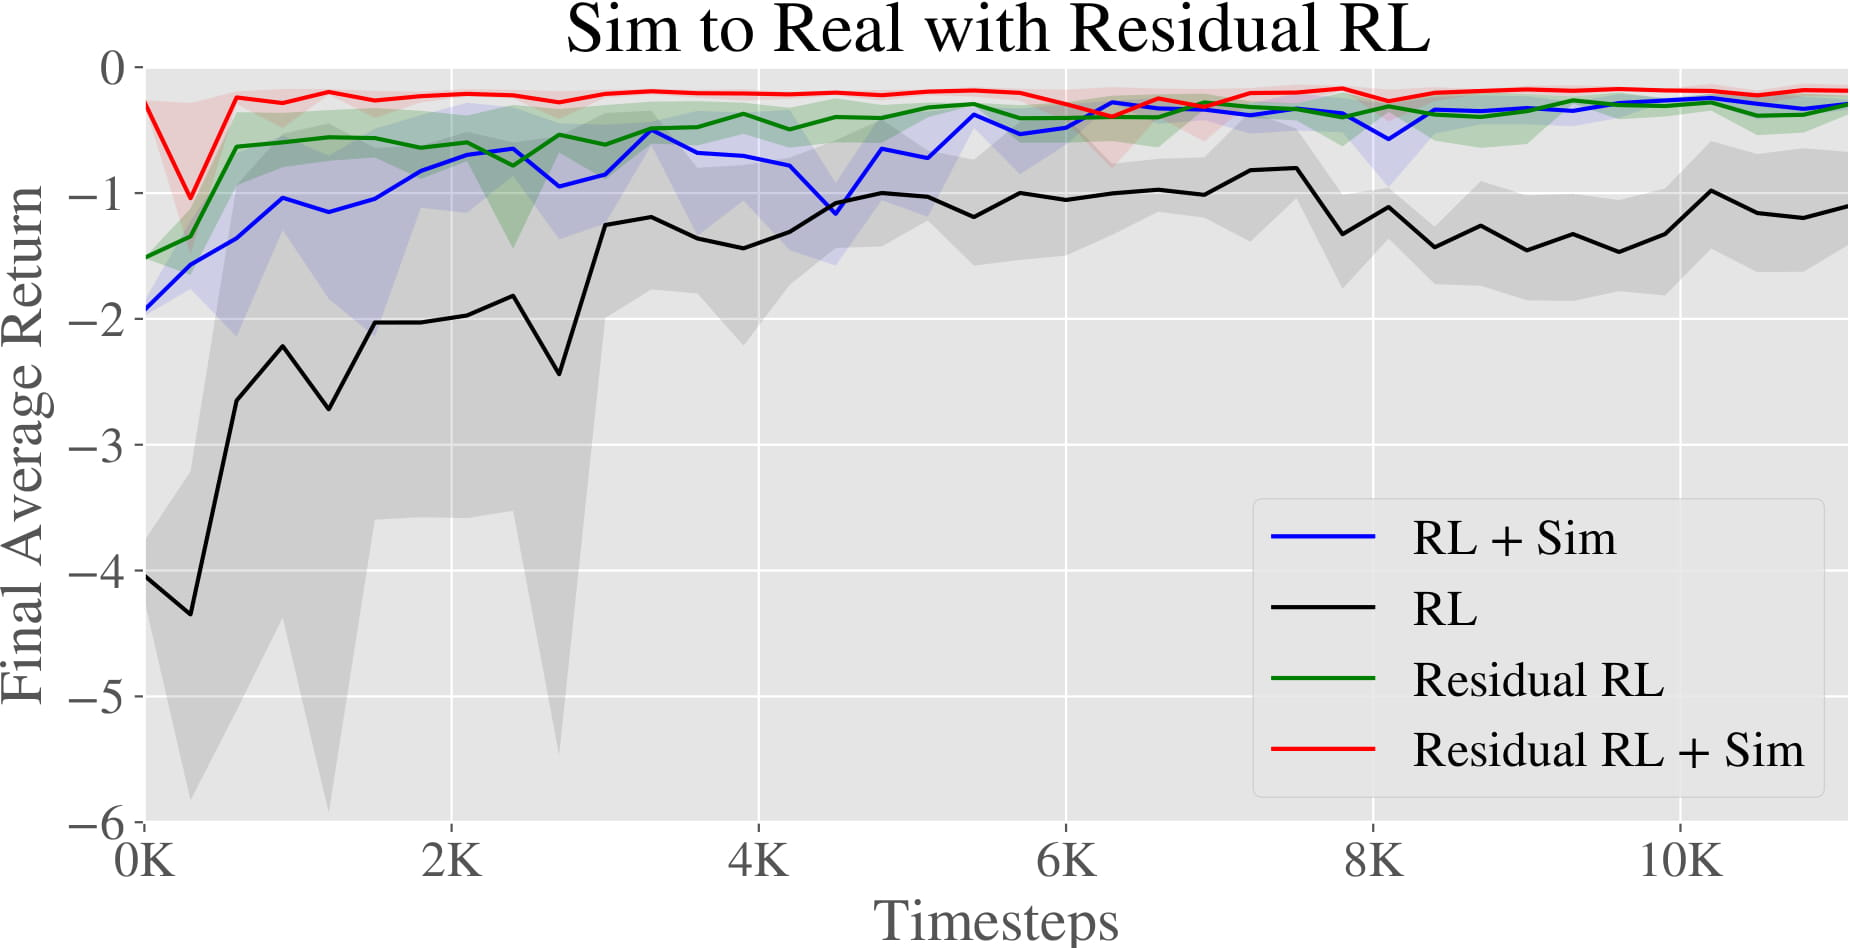
\includegraphics[width=0.99\linewidth]{residualrl/figs/sim_to_real_bitmap.jpg} \\
    \centering
    \captionsetup{justification=justified,format=plain}
    \caption{Real-world block insertion results using residual RL for sim-to-real transfer. ``Sim'' indicates that the real-world policy was initialized by reinforcement learning in simulation. Residual RL with simulation initialization successfully solves the task with little environment experience required. } %
    \label{fig:sim_to_real}
\end{wrapfigure}
%\newpage
Often, intensive reward shaping is key for RL to succeed at a task and prior work has even considered reward shaping as part of the learning system \cite{daniel2014activereward}. Reward shaping in order to tune agent behavior is a very manual process and recovering a good policy with reward shaping can be as difficult as specifying the policy itself. Hence, in our method we allow for human specification of both rewards and policies---whichever might be more practical for a particular task.

Further work has incorporated more specialized human knowledge into RL systems. One approach is to use trajectory planners in RL in order to solve robotics tasks \cite{thomas2018cad}. However, since the method optimizes trajectory following instead of the task reward, generalization can be difficult when aspects of the environment change. Other work has focused on human feedback \cite{loftin2014discretehumanfeedback, saunders2018trialwithouterror, torrey2013teachingbudget, frank2008rareevents, christiano2017humanpreferences} to inform the agent about rewards or to encourage safety. However, in many robotics tasks, providing enough information about the task through incremental human feedback is difficult.

Another way to include prior knowledge in RL is through demonstrations~\cite{peters2008baseball, kober2008mp, rajeswaran2018dextrous, hester17dqfd, vecerik17ddpgfd, nair2018demonstrations}. Demonstrations can substantially simplify the exploration problem as the agent begins training having already received examples of high-reward transitions and therefore knows where to explore \cite{subramanian2016efd}. However, providing demonstrations requires humans to be able to teleoperate the robot to perform the task. In contrast, our method only requires a conventional controller for motion, which ships with most robots.

Prior knowledge can also be induced through neural network architecture choices. Deep residual networks with additive residual blocks achieved state of the art results in many computer vision tasks by enabling training of extremely deep networks \cite{he2016resnet}. In RL, structured control nets showed improvement on several tasks by splitting the policy into a linear module and a non-linear module \cite{srouji18structuredcontrolnets}. Prior work in adaptive flight control has also considered compensating linearized controllers with neural networks \cite{johnson2000hedging}. Most closely related to our work, residual policy learning concurrently and independently explores training a residual policy in the context of simulated long-horizon, sparse-reward tasks with environment variation and sensor noise \cite{silver18residualpolicylearning}. Our work instead focuses on achieving practical real-world training of contact-intensive tasks.
